\documentclass{beamer}

\usepackage{default}
\usepackage[utf8]{inputenc}
\usepackage[T1]{fontenc}
%\usepackage[ngerman]{babel}
\usepackage{enumerate}
\usepackage{listings}
\usepackage{marvosym}
\usepackage{gensymb}
\usepackage{graphicx}

\usepackage[nodayofweek]{datetime}
\usepackage{hyperref}
\usepackage{breakurl}


\usepackage{amsmath}
\usepackage{amsfonts}
\usepackage{amssymb}
\usepackage{thmtools}

%\newtheorem{definition}{Definition}
%\newtheorem{proposition}{Propsition}
%\newtheorem{proof}{Proof}
\newtheorem{axiom}{Axiom}



\graphicspath{{./images/}}

\usetheme{metropolis}
%\usecolortheme{beetle}


\title{Trace Link Recovery \\using Static Program Analysis}
\subtitle{\it B.Sc. Thesis Colloquium/Defense}
\author{Maximilian Meffert}
\institute{University of Koblenz-Landau}
\date{\today}

\beamertemplatenavigationsymbolsempty 
\setbeamertemplate{bibliography item}[text]

\makeatother
\setbeamertemplate{footline}[text line]{
\parbox{\linewidth}{
\vspace*{-8pt}
\tiny
\insertshorttitle
\hfill
\insertshortauthor
\hfill
\insertshortinstitute
\hfill
}}
\makeatletter

\newcommand{\partOf}{~\textsf{partOf}~}
\newcommand{\properPartOf}{~\textsf{properPartOf}~}
\newcommand{\Any}{~\textsf{Any}~}
\newcommand{\correspondsTo}{~\textsf{correspondsTo}~}
\newcommand{\correspondsToR}[1]{~\textsf{correspondsTo}_{#1}~}
\newcommand{\conformsTo}{~\textsf{conformsTo}~}


\newcommand{\megal}{\text{MegaL}}
\newcommand{\megalxtext}{\text{MegaL/Xtext}}
\newcommand{\megaltext}{\text{MegaL/Text}}
\newcommand{\eclipse}{\text{eclipse}}


\definecolor{anti-flashwhite}{rgb}{0.95, 0.95, 0.96}
\lstset{
basicstyle=\tiny,
morekeywords={company,Company,id},
keywordstyle=\itshape\color{red},
backgroundcolor=\color{anti-flashwhite}
}

\begin{document}

\frame{\titlepage}

\begin{frame}{General Information}
\centering
\textbf{Maximilian Meffert}\\~\\
\resizebox{\textwidth}{!}{
\begin{tabular}{ll}
Mat.-Nr.: & 210 101 205\\
E-Mail: & \href{mailto:maxmeffert@uni-koblenz.de}{maxmeffert@uni-koblenz.de}\\
GitHub: & \url{https://github.com/maxmeffert}\\
Thesis-Repo.: & \url{https://github.com/maxmeffert/BScThesis}
\end{tabular}
}
\\~\vspace{\fill}~\\
\textbf{Supervisors}\\~\\
\resizebox{\textwidth}{!}{
\begin{tabular}{ll}
Prof. Dr. Ralf Lämmel 
& University of Koblenz-Landau, \textit{Institute for Computer Science} \\
M.Sc. Johannes Härtel 
& University of Koblenz-Landau, \textit{Institute for Computer Science}
\end{tabular}
}
\end{frame}

\begin{frame}{Motivation: Software as Cognitive Challenge}
\begin{columns}
\begin{column}{0.5\textwidth}
\begin{center}
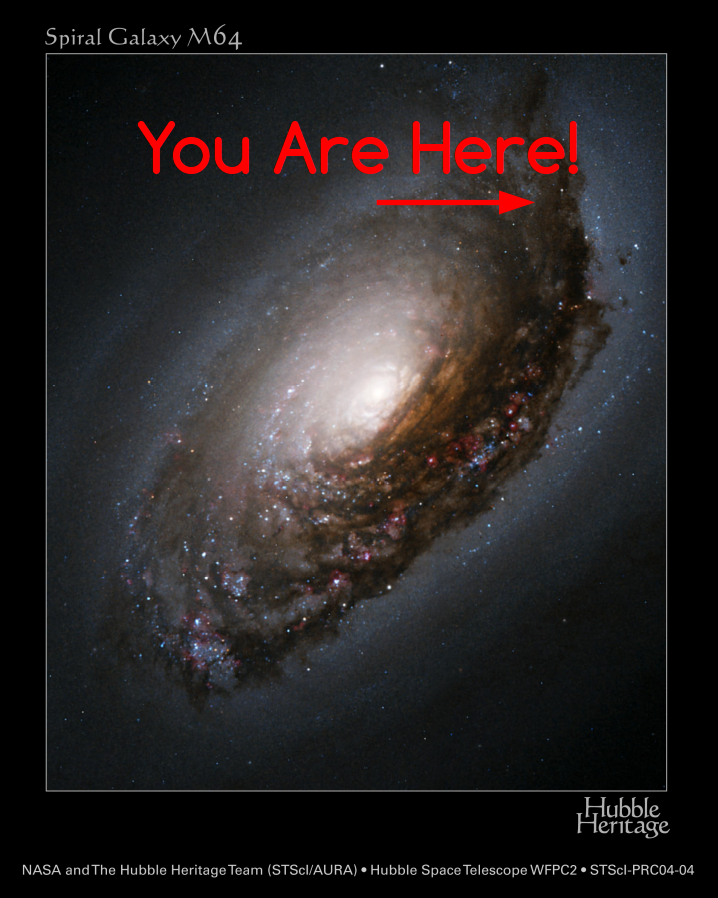
\includegraphics[width=\textwidth]{YouAreHere.png}
\newline
\footnotesize
View on the "Black Eye" galaxy provided by \cite{BlackEyeGalaxy}.
\end{center}
\end{column}
\begin{column}{0.5\textwidth}
Modern Software Systems are:
\begin{itemize}
\item
large\\(allover artifact count)
\item
heterogeneous\\(languages involved)
\end{itemize}
$\Rightarrow$
challenging for program comprehension tasks 
\end{column}
\end{columns}
\end{frame}

\begin{frame}[fragile,allowframebreaks]{Traceability}
asdf
\end{frame}

\begin{frame}[fragile,allowframebreaks]{Traceability Terminology}
\begin{definition}[Trace]
\begin{description}[align=left]
\item[(Noun)]
A specified triplet of elements comprising: \emph{source artifact}, \emph{target artifact} and a \emph{trace link} associating the two \emph{trace artifacts}. \cite{DBLP:books/daglib/p/GotelCHZEGDAMM12}
\item[(Verb)]
The act of following a trace link. \cite{DBLP:books/daglib/p/GotelCHZEGDAMM12}
\end{description}
\end{definition}
%\begin{definition}[Trace Link]
%A specified association between a pair of artifacts, on comprising the soruce artifact and on comprising the target artifact. 
%\cite{DBLP:books/daglib/p/GotelCHZEGDAMM12}
%\end{definition}

\end{frame}

\begin{frame}{Linguistic Architectures}
%\cite{DBLP:books/daglib/p/GotelCHZEGDAMM12}
\end{frame}

\begin{frame}[fragile,allowframebreaks]{Trace Link Recovery Approach}
\begin{center}
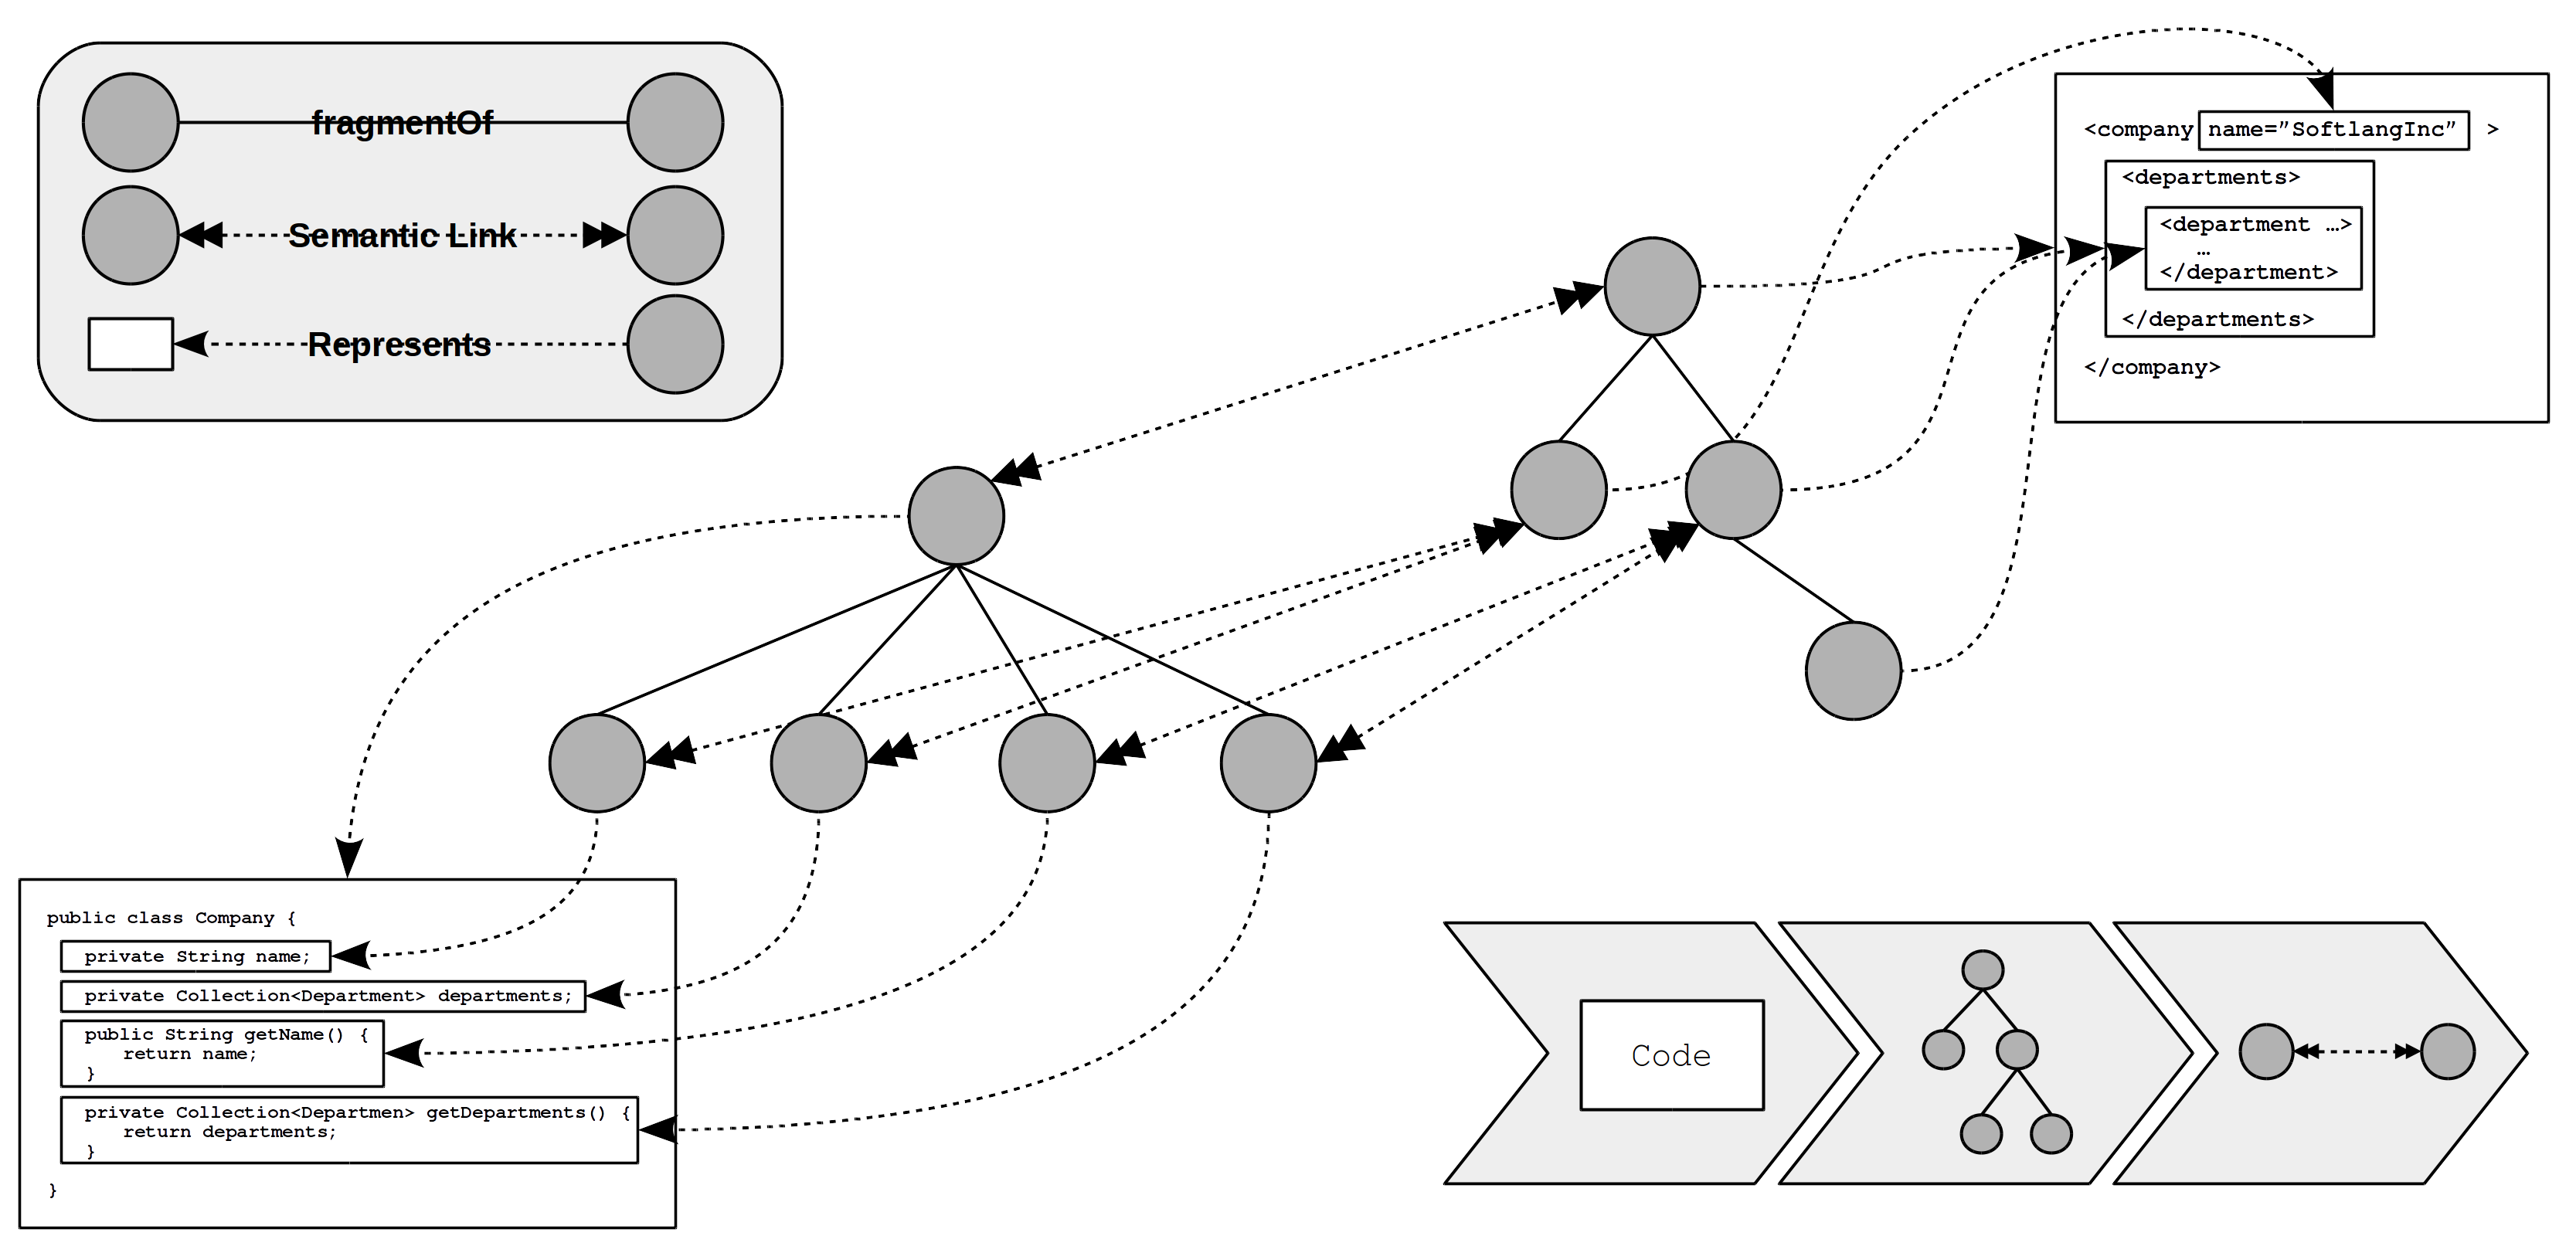
\includegraphics[width=\textwidth]{RecoveryApproach.png}
\end{center}
\pagebreak
asdf
\end{frame}



\begin{frame}{References}
\bibliographystyle{splncs}
\bibliography{bibliography}{}
\end{frame}


\end{document}
